\chapter{Metodologia ed architettura}
La metodologia adoperata fa uso di un database \emph{NoSQL}, per il mantenimento dei dati, e della tecnologia \emph{Apache Spark} su macchina virtuale \emph{Azure}.\par 
La macchina virtuale mette a disponizione:
\begin{itemize}
	\item 8 core
	\item Memoria centrale di 58 GB
	\item Memoria di massa di 30 GB
	\item Disco temporaneo secondario di 400 GB
\end{itemize}
Accessibile mediante protocollo SSH, offre l'utilizzo dell'engine Apache Spark con stack relativo già installato e configurato. In particolare si è fatto uso del modello di programmazione Spark per il linguaggio Python: \emph{Pyspark}.\par
Il database NoSQL utilizzato è \emph{MongoDB} per la tipologia di dati da trattare e le operazioni da effettuare su di essi. MongoDB è un database documentale che consente di trattare aggregati strutturati, risultando in accessi più flessibili. Permette, quindi, di sottomettere query basate sui campi dell'aggregato e recuperare solo parte di esso. MongoDB memorizza e restituisce documenti in formato \emph{BSON}, rappresentazione binaria del JSON. I documenti sono strutture dati ad albero gerarchiche e possono essere anche strutturalmente non identici. Sono infatti distinti per collezione, insieme di documenti simili. Le caratteristiche di MongoDB hanno consentito una gestione semplice ed efficace del dataset composto principalmente da file \emph{JSON} e \emph{XML}. Il flessibile modello documentale dei dati con schema dinamico e ridimensionamento automatico su hardware comune rende MongoDB ideale per applicazioni con grandi volumi di dati multi-strutturati e dall'elevato tasso di cambiamento. Inoltre MongoDB offre la completa interoperabilità con il sistema Spark, mediante il \emph{MongoDB Spark Connector}, che ne consente la gestione tramite codice Pyspark.

\begin{figure}[H]
	\centering
	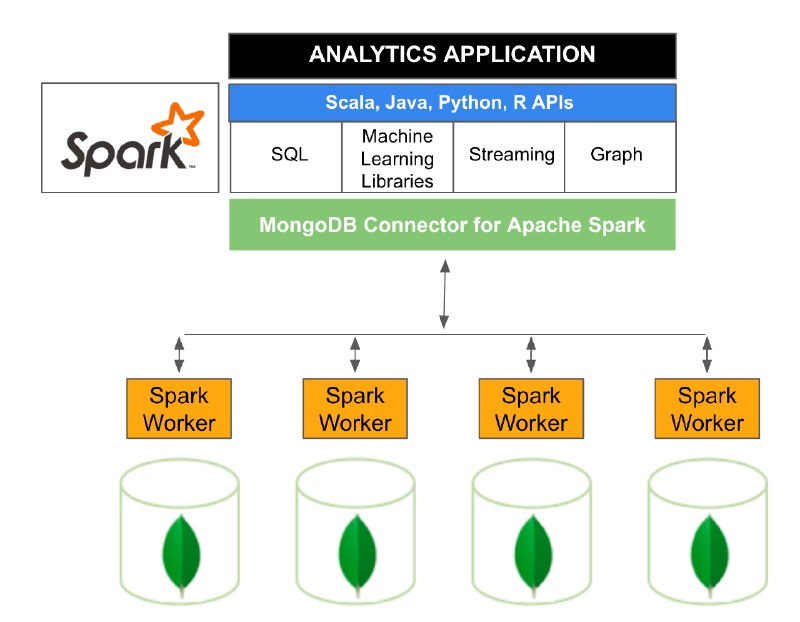
\includegraphics[scale=0.5]{./image/mongospark.jpg}
	\caption{MongoDB Spark Connector}
	\label{fig:msc}
\end{figure}

Apache Spark è un framework di data processing che consente di effettuare query veloci grazie alla memorizzazione \emph{in-memory} dei dati. Supporta diversi linguaggi di programmazione: Scala, Java, R, Python. Le sue principali caratteristiche sono:
\begin{description}
	\item[Velocità] sfruttando le ottimizzazioni in-memory;
	\item[Framework unificato] offrendo packages di librerie di alto livello (supporto a query SQL, Machine Learning, stream e graph processing);
	\item[Semplicità] includendo API facili da usare per operare su grandi dataset, come operatori per trasformare e manipolare dati semistrutturati.
\end{description}
Spark, combinato con Python, è stato sfruttato sia per il caricamento del dataset di file XML nel database, non nativamente convertibile in BSON da MongoDB, sia per l'elaborazione dei dati.\par 
L'unione di queste due tecnologie consente allo sviluppatore di realizzare l'applicazione più velocemente, utilizzando un solo database. Spark può eseguire direttamente sui dati operativi posti in MongoDB, senza tempi e costi di un processo di ETL. MongoDB può efficientemente presentare di ritorno i risultati analitici ai processi operativi.

\begin{figure}[H]
	\centering
	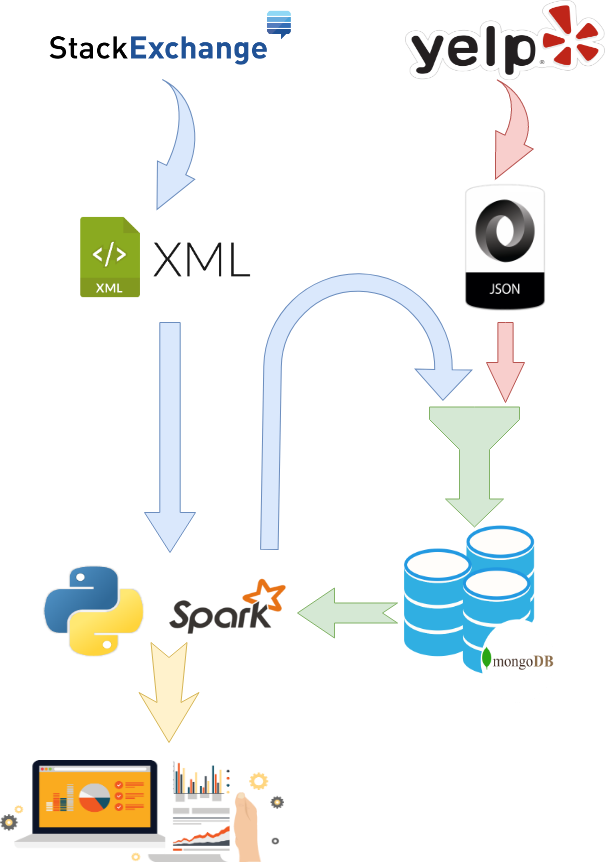
\includegraphics[scale=0.5]{./image/BDABI.png}
	\caption{Architettura}
	\label{fig:arc}
\end{figure}